\begin{fact} \label{ortho-rebond}
	Supposons que $\sigma_S = 0$.
	
	\medskip
	
	Notant $M$ l'intersection de $(SH_S)$ avec $\geoset*{d}{1}$, nous avons que $M$ est sur le trajet de la bille avec $\sigma_M < 0$
	\footnote{
		On pourrait avoir un résultat plus fin mais ceci ne nous serait inutile pour la suite.
	}.
\end{fact}

\begin{proof}
	Évident grâce au dessin précédent.
\end{proof}


\medskip


\begin{fact} \label{deux-rebonds-vers-F}
	Supposons que $\sigma_S \in \intervalO{0}{\dfrac{\pi}{2} - \theta + \tau}$.
	
	\medskip
	
	Il existe un point $M$ sur le trajet de la bille, mais pas sur $\geoset*{d}{1}$, tel que $\sigma_M  < 0$.
\end{fact}

\begin{proof}
	Au bout de deux rebonds, nous avons trois situations possibles dont les deux premières ci-après ne nécessitent aucune explication.
	
	
	\medskip
	
	\begin{center}
		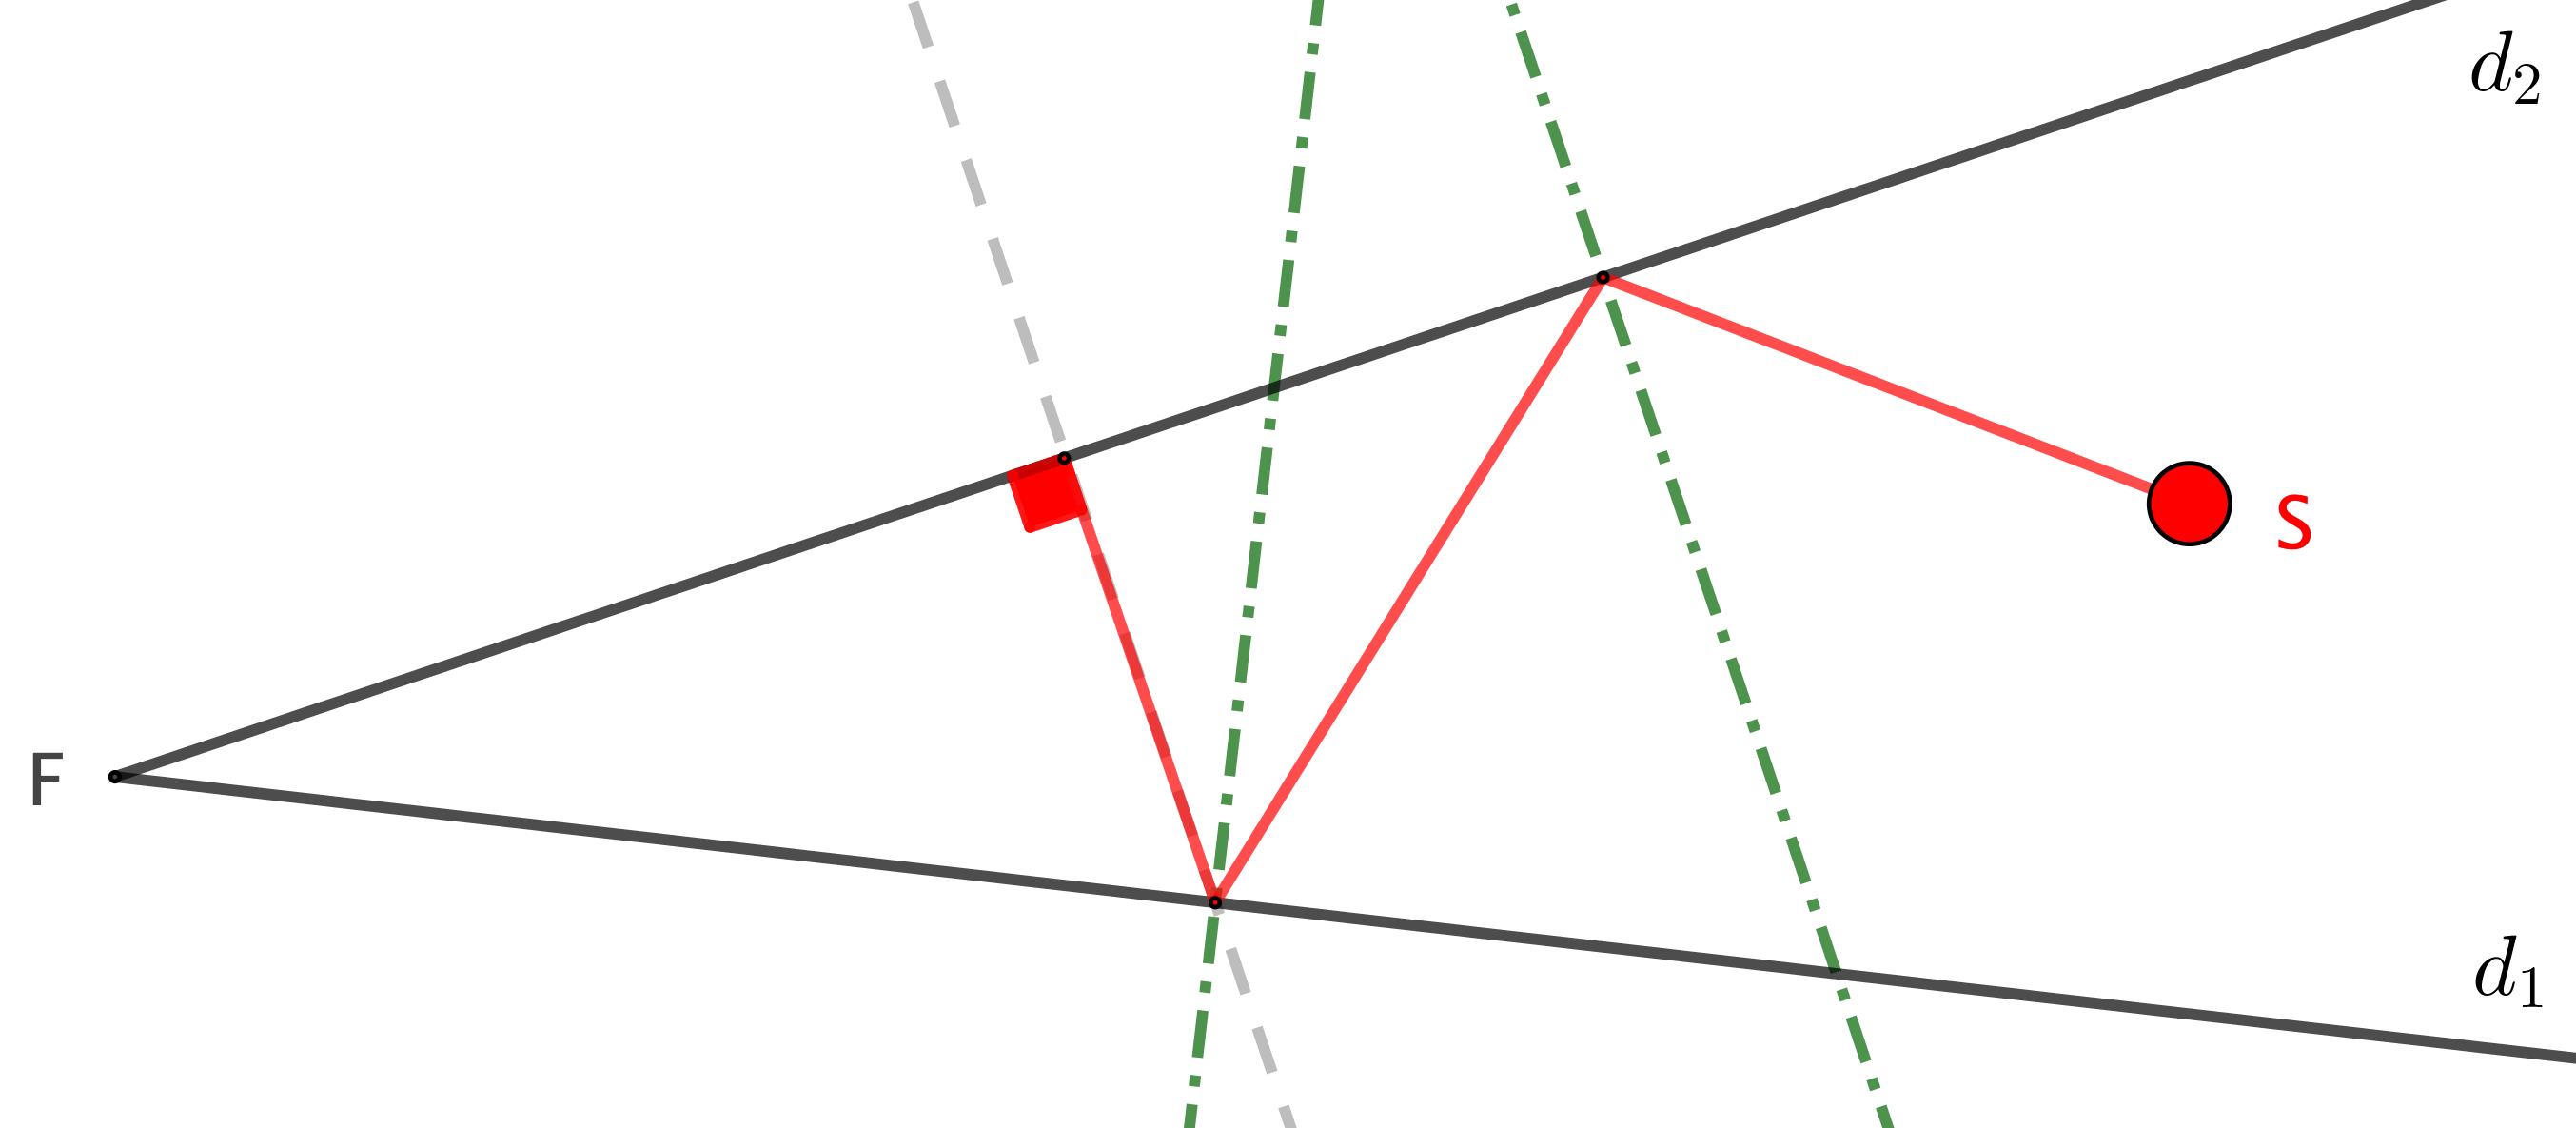
\includegraphics[width=12cm]{basic-math-pool/proof-starting-with-d2-2-bounces-to-ortho.png}

		\itshape\small
		Le 2\ieme{} rebond nous ramène à la situation du fait \ref{ortho-rebond} ci-dessus
		
		qui nous permet de conclure directement.
	\end{center}
	
	
	\medskip
	
	\begin{center}
		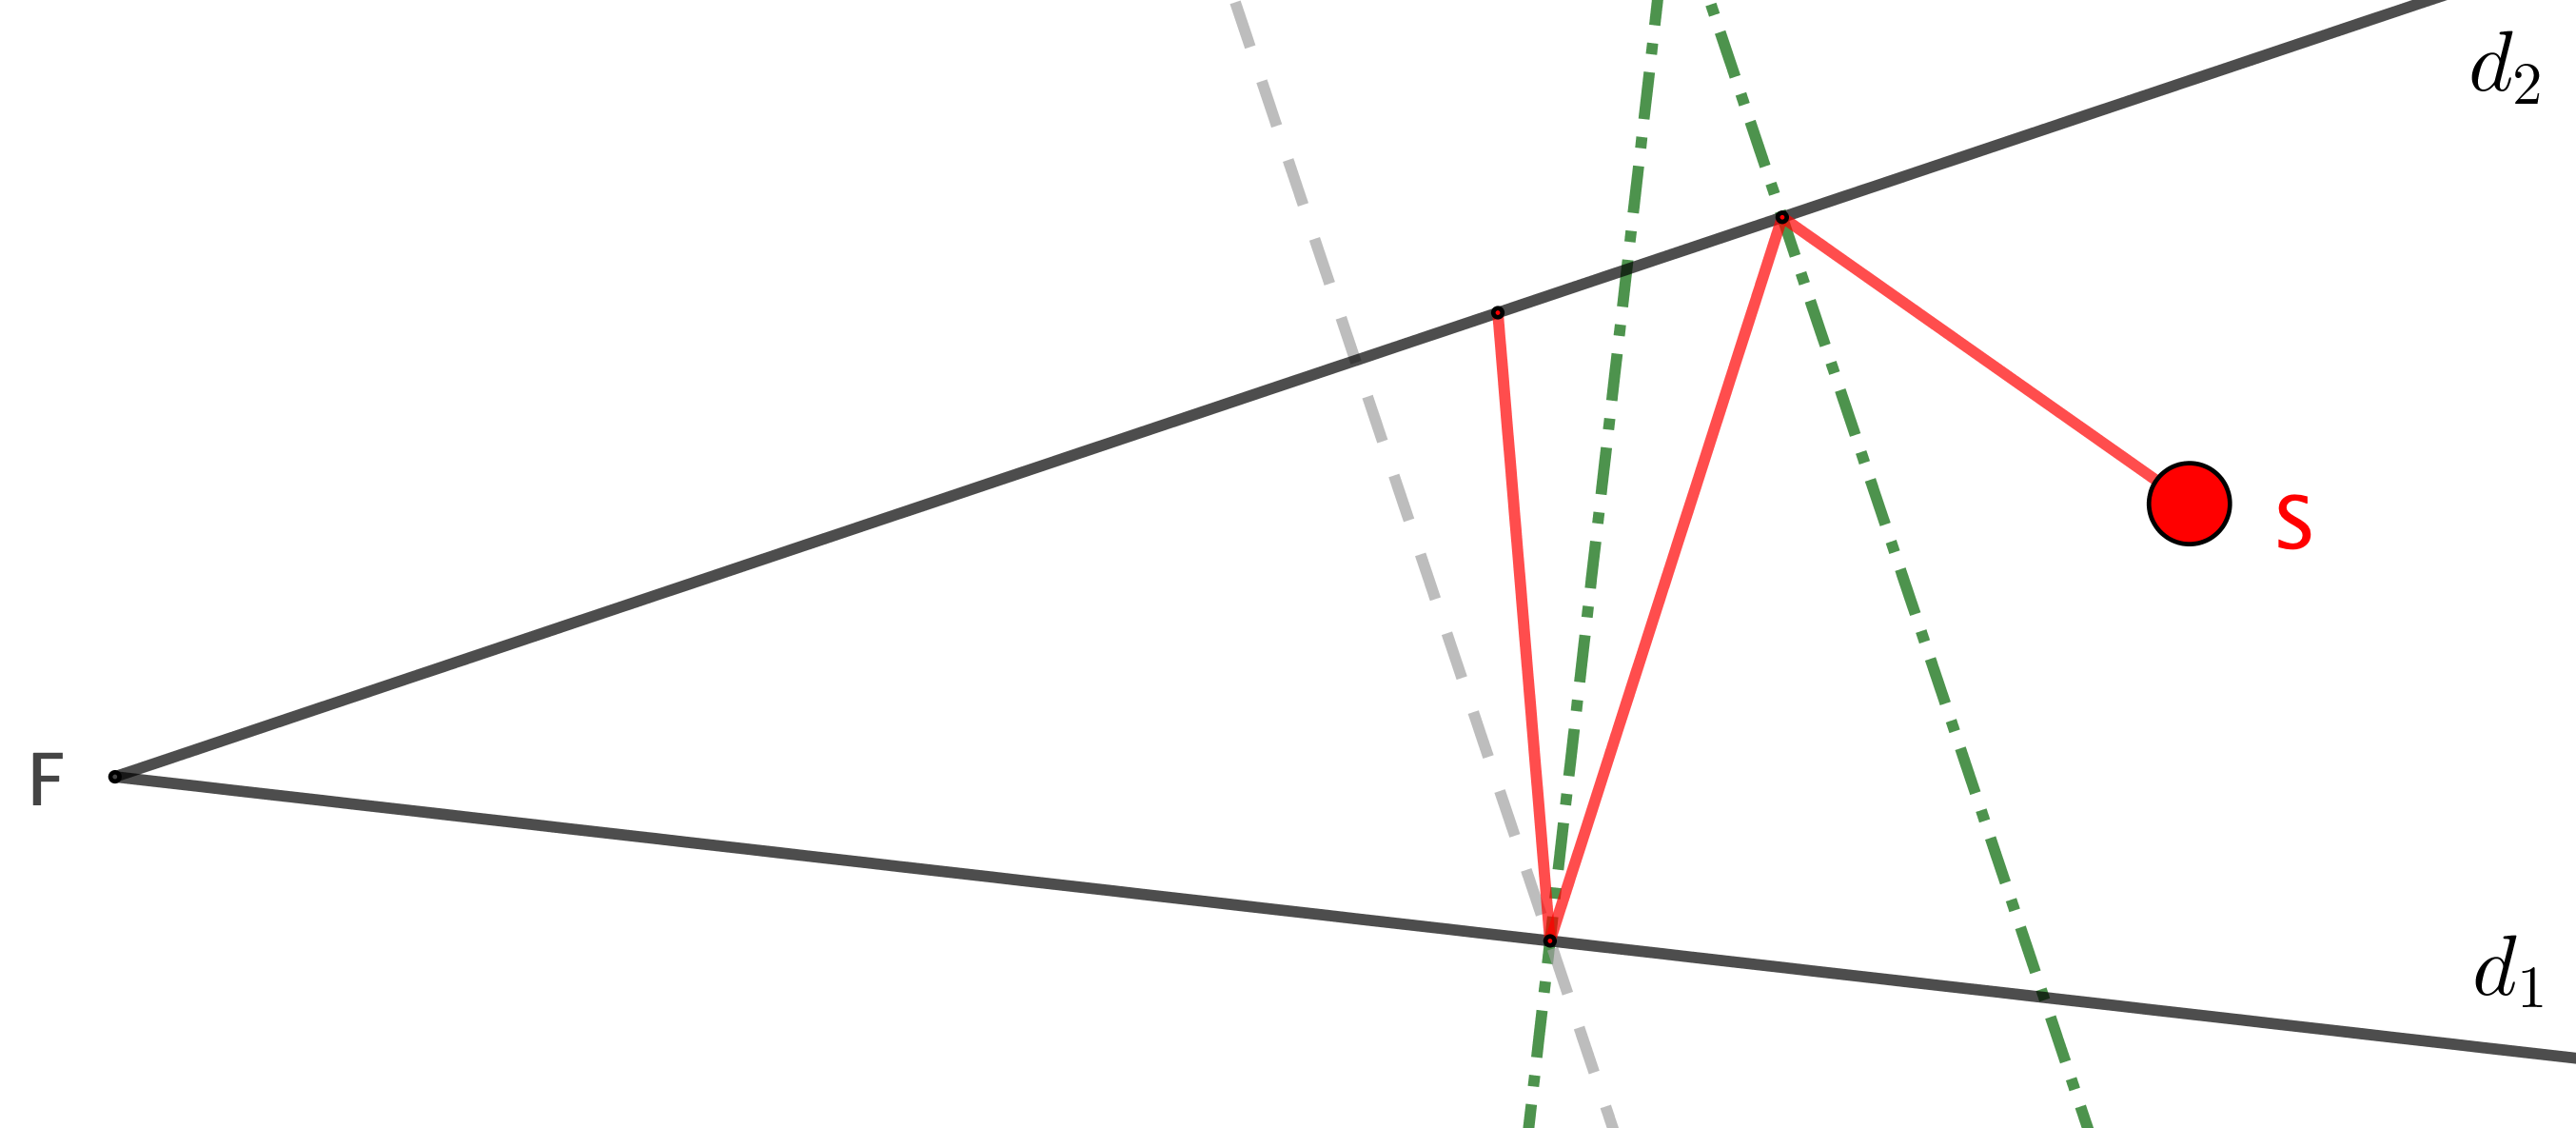
\includegraphics[width=12cm]{basic-math-pool/proof-starting-with-d2-2-bounces-to-infinity.png}

		\itshape\small
		Le 2\ieme{} rebond nous ramène directement à la bonne situation.
	\end{center}
	
	
	\medskip
	
	Voici la dernière situation représentée ci-dessous où $\geoset{D}_2 \, /\!/ \, \geoset{d}_2$.
	
	
	\medskip
	
	\begin{center}
		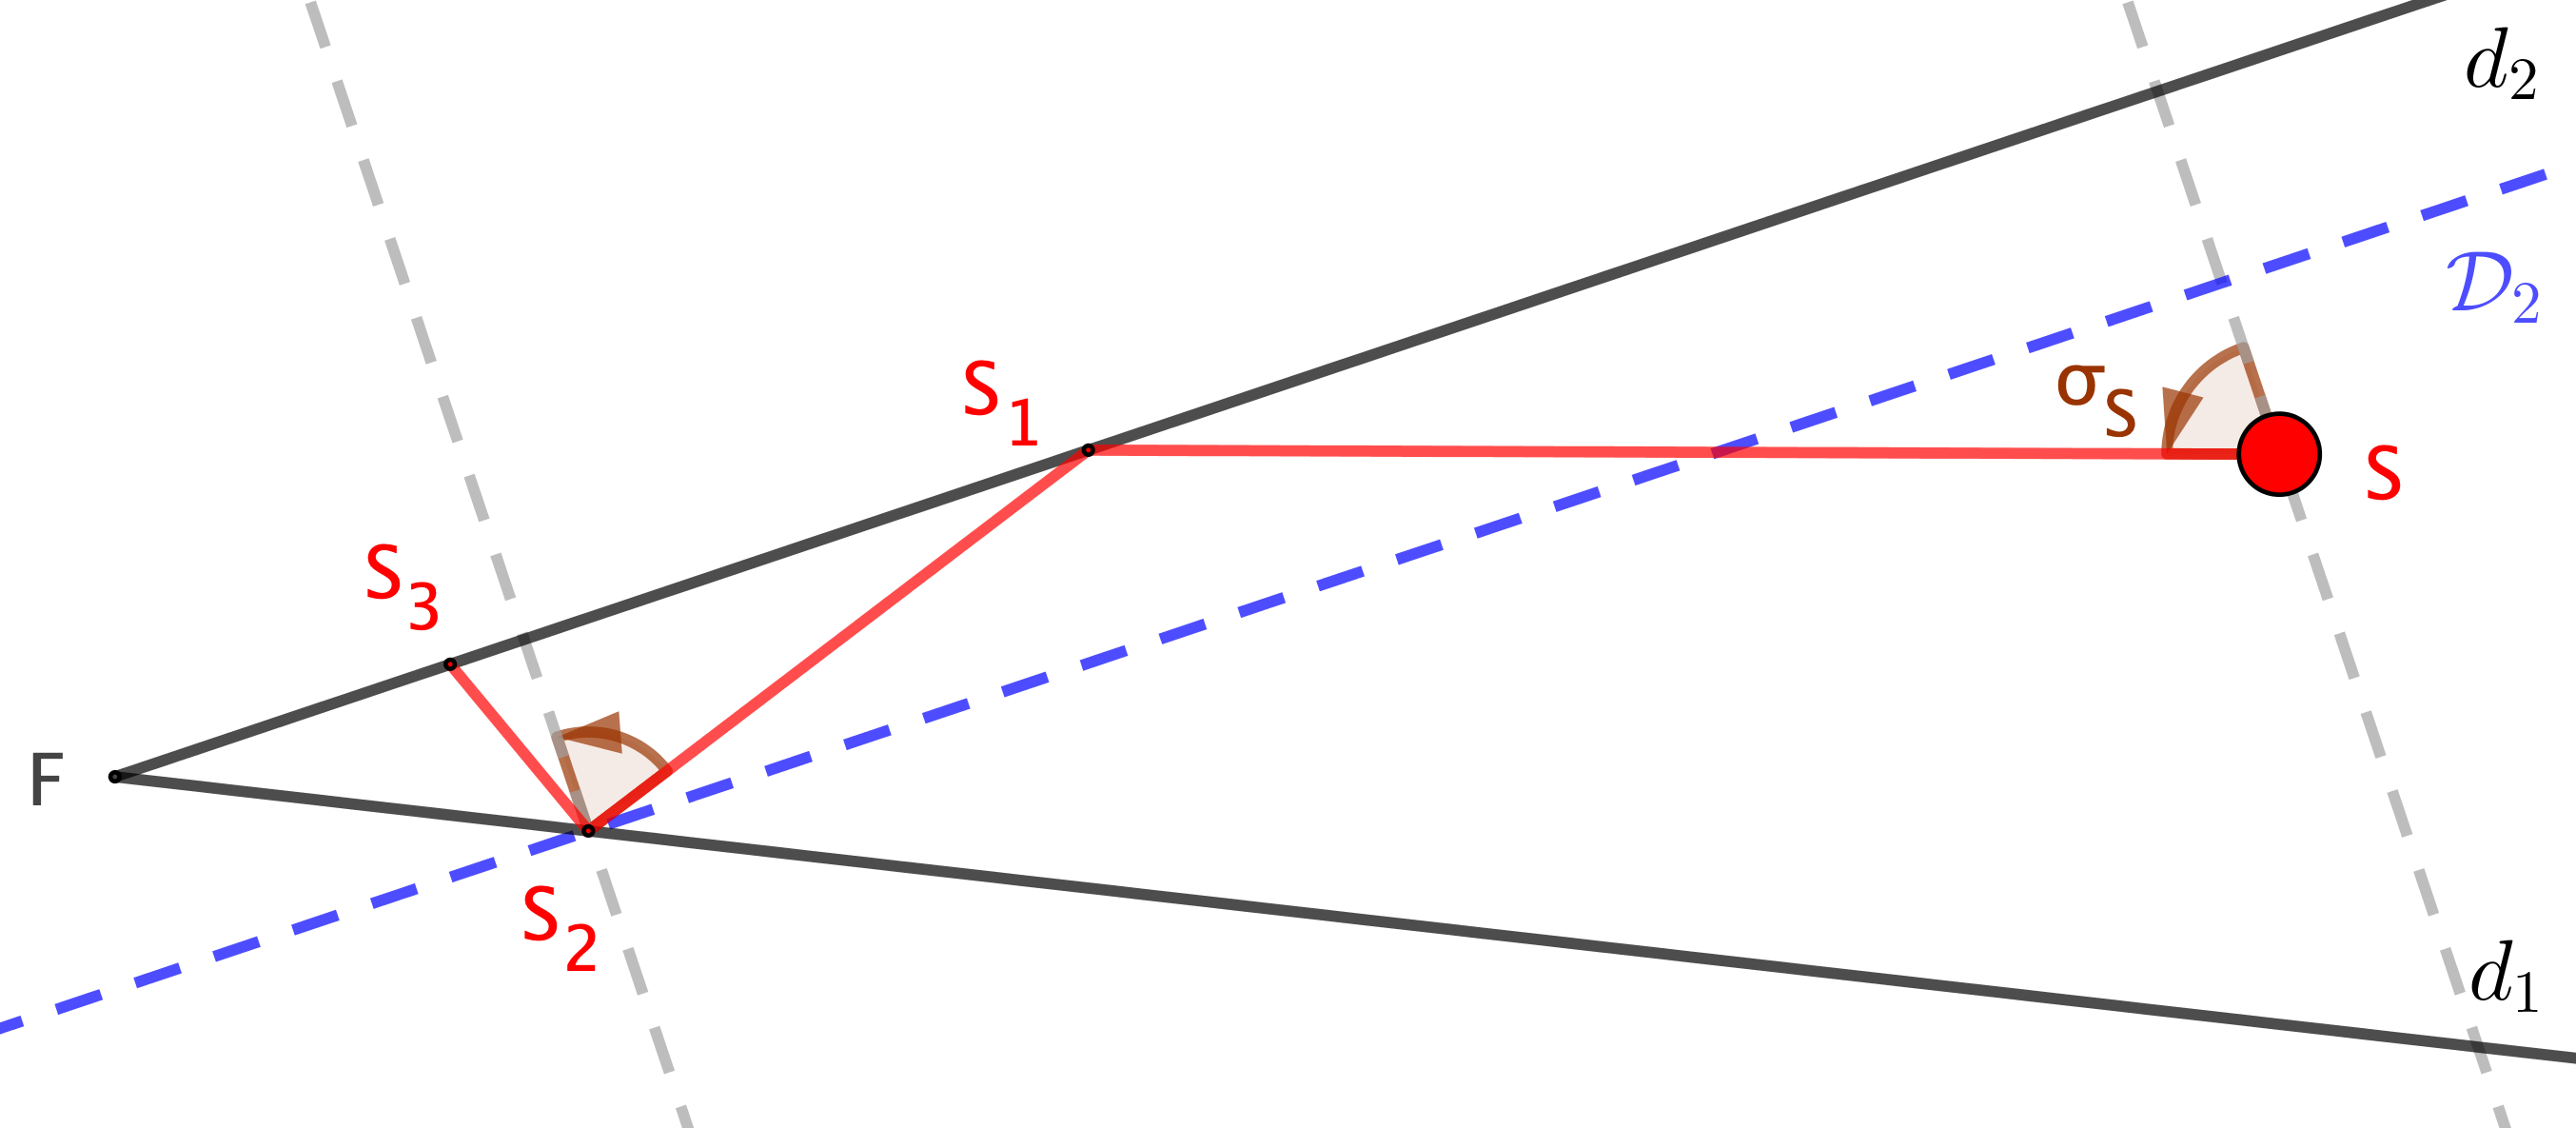
\includegraphics[width=12cm]{basic-math-pool/proof-starting-with-d2-2-bounces-to-F.png}

		\itshape\small
		Le 2\ieme{} rebond nous ramène à la situation de départ
		
		mais avec une valeur de $\sigma$ qui a augmenté.
	\end{center}
	
	
	\medskip
	
	Faisons un zoom sur la partie de gauche pour évaluer précisément l'évolution faisant passer de $\sigma_S$ à $\sigma_{S_2}$.
	
	\begin{center}
		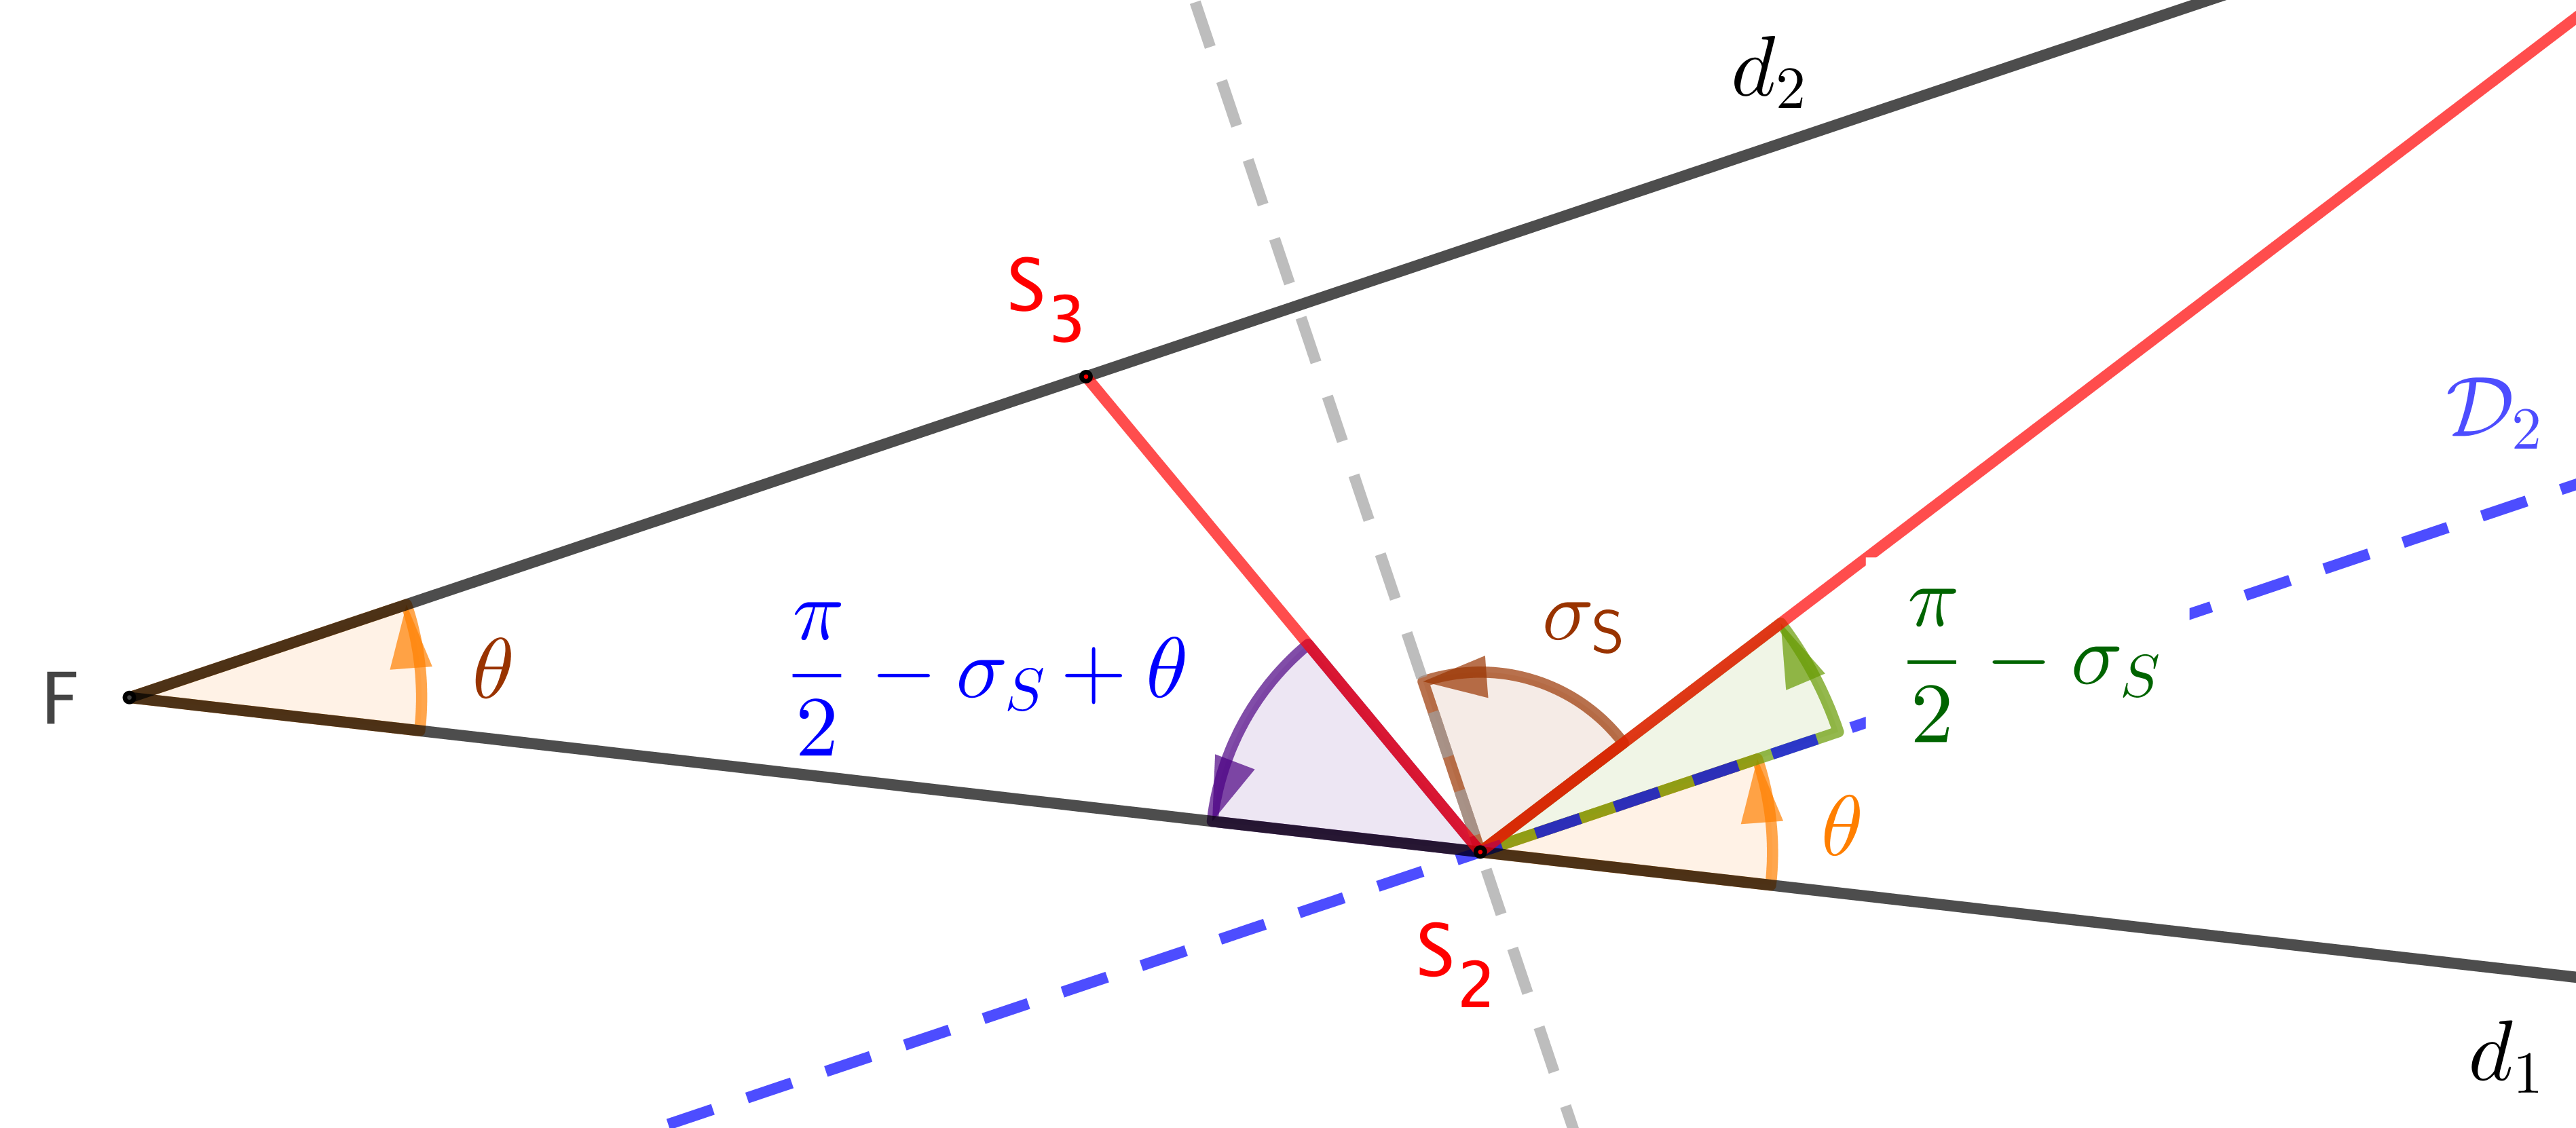
\includegraphics[width=12cm]{basic-math-pool/proof-starting-with-d2-2-bounces-to-F-zoom.png}
	\end{center}
	
	
	\medskip
	
	Nous avons alors $\sigma_{S_2} = \pi - 2 \left( \dfrac{\pi}{2} - \sigma_S + \theta \right) - \sigma_S = \sigma_S - 2 \theta$.
	Ceci montre que l'on passe de $\sigma_S$ à $\sigma_{S_2} = \sigma_S + \delta$ où $\delta = - 2 \theta < 0$. Cette dernière relation montre que l'on ne pourra pas avoir indéfiniment la dernière situation \emph{(en toute rigueur, il faudrait faire un raisonnement par récurrence)}.  
\end{proof}


\medskip


\begin{fact} \label{s-eloigner}
	Supposons que $\sigma_S \in \intervalCO{- \dfrac{\pi}{2}}{0}$.

	\medskip
	
	Il existe un point $M$ sur le trajet de la bille, mais pas sur $\geoset*{d}{1}$, tel que $\sigma_M < - \dfrac{\pi}{2}$. En particulier, à partir de ce point $M$ la bille s'éloignera indéfiniment loin de $F$.
\end{fact}

\begin{proof}
	La démarche est similaire à la preuve précédente.
	Pour la situation problématique, on utilise les deux graphiques donnés dans la page suivante qui nous montrent que l'on passe de $\sigma_S$ à $\sigma_{S_2} = \sigma_S + \delta$ où $\delta = - 2 \theta < 0$. Ceci nous permet une seconde fois de conclure puisque l'on ne pourra pas avoir indéfiniment $\sigma_{S_{2k}} \geqslant - \dfrac{\pi}{2}$.
\end{proof}


\medskip


\begin{theorem}
	Si le 1\ier{} rebond se fait sur $\geoset*{d}{2}$ alors il n'y aura qu'un nombre fini de rebonds et le dernier rebond amènera la bille à s'éloigner indéfiniment loin de $F$.
\end{theorem}

\begin{proof}
	Distinguons trois cas.
	
	\begin{itemize}[label = \textbullet]
		\item Si $\sigma_S \in \intervalCO{- \dfrac{\pi}{2}}{0}$ alors tout est donné par le fait \ref{s-eloigner}.


		\item Si $\sigma_S = 0$ alors le fait \ref{ortho-rebond} nous donne un point $M$ sur le trajet de la bille, mais pas sur $\geoset*{d}{1}$, tel que $\sigma_M < 0$.
		
		\noindent
		Si $\sigma_M < - \dfrac{\pi}{2}$, nous savons qu'à partir de $M$ la bille s'éloignera indéfiniment loin de $F$.
		
		\noindent
		Sinon nous avons $\sigma_M \in \intervalCO{- \dfrac{\pi}{2}}{0}$.
		Le fait \ref{s-eloigner} nous permet alors de conclure.
		
		
		\item Enfin si $\sigma_S \in \intervalO{0}{\dfrac{\pi}{2} - \theta + \tau}$, il suffit de raisonner comme dans le point précédent mais en invoquant le fait \ref{deux-rebonds-vers-F}.
	\end{itemize}
\end{proof}

	
\medskip


\begin{center}
	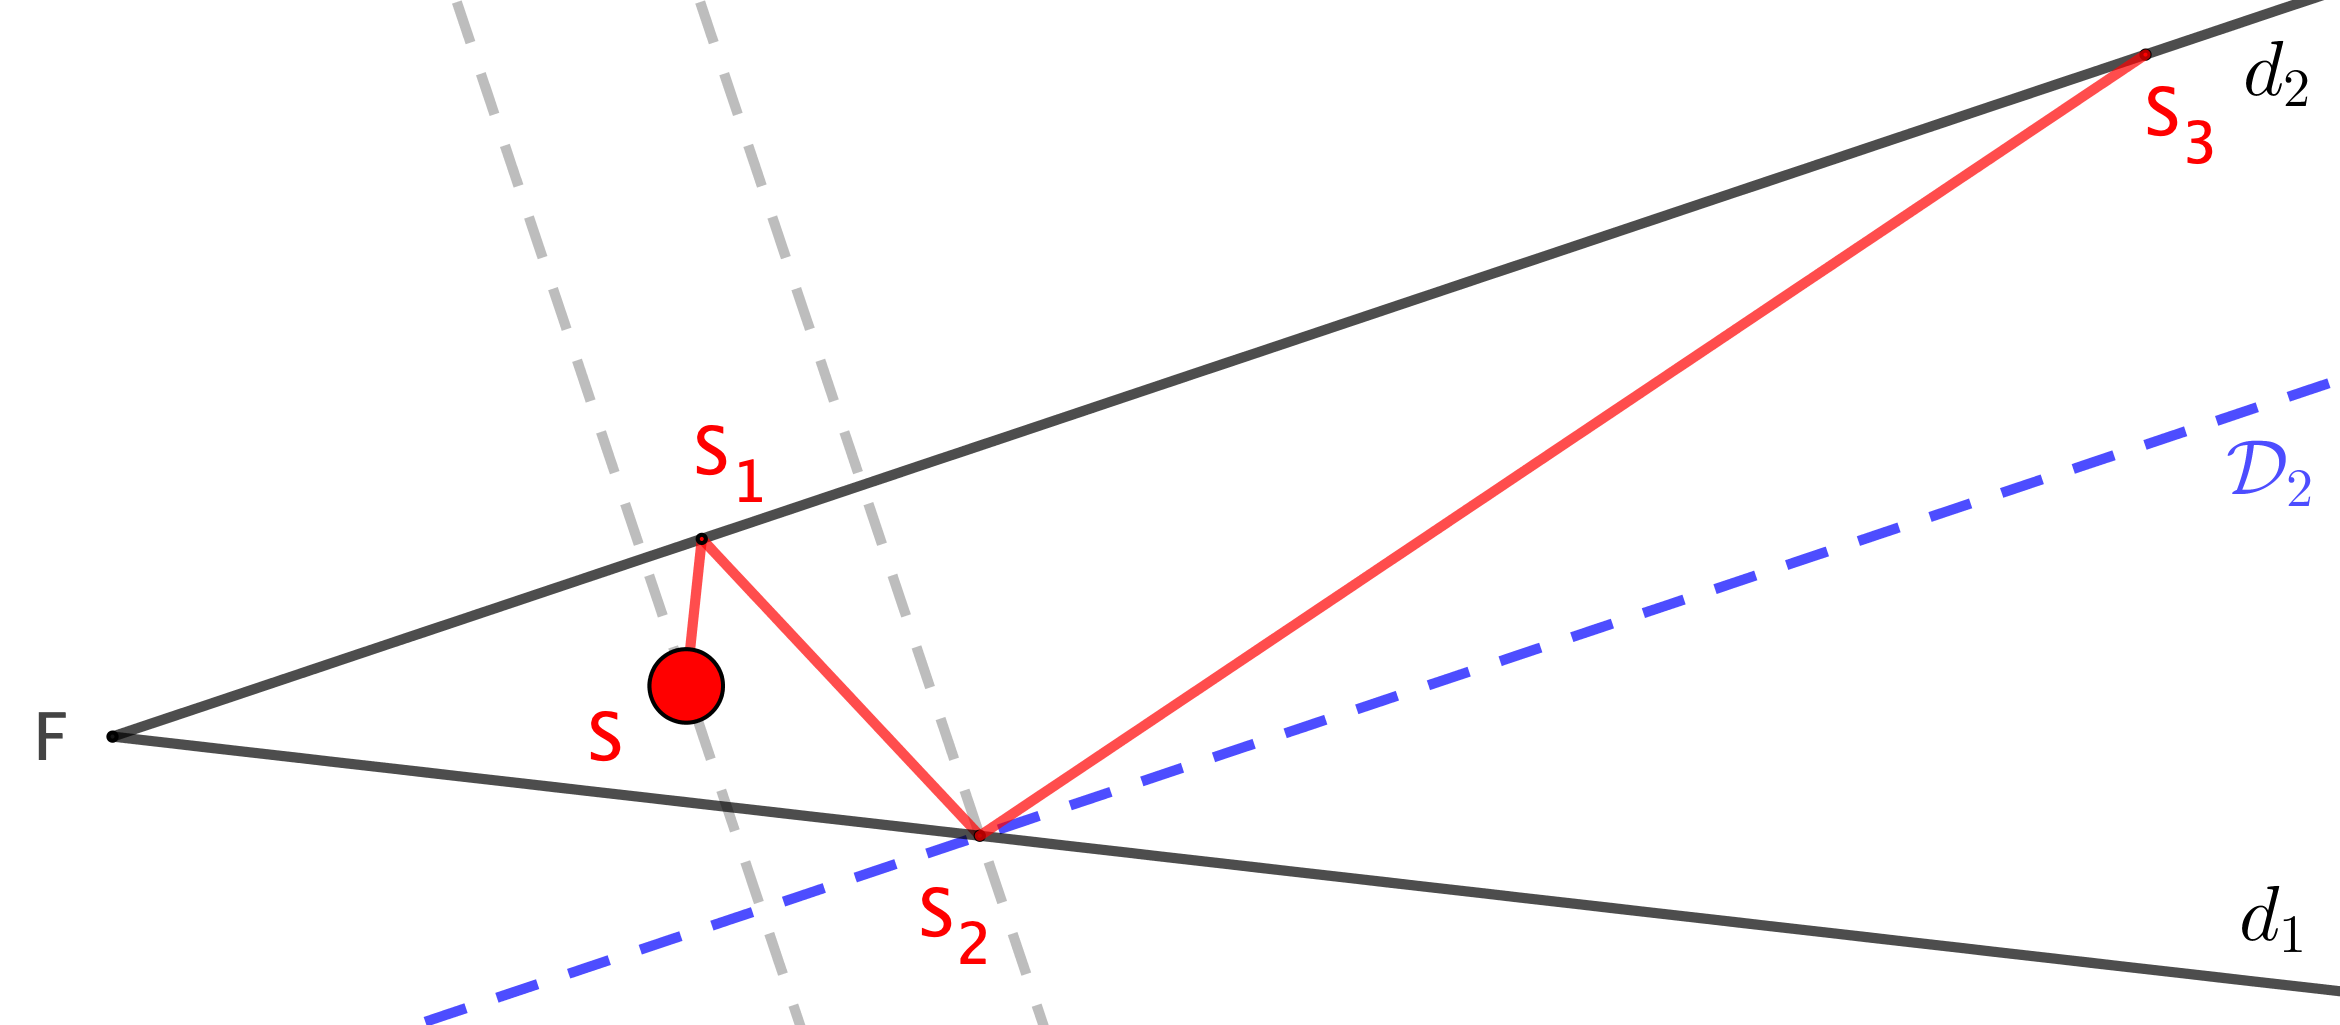
\includegraphics[width=12cm]{basic-math-pool/proof-starting-with-d2-2-bounces-farway-from-F.png}

	\itshape\small
	Preuve du fait \ref{s-eloigner} -- Vue large du cas problématique
\end{center}

	
\medskip


\begin{center}
	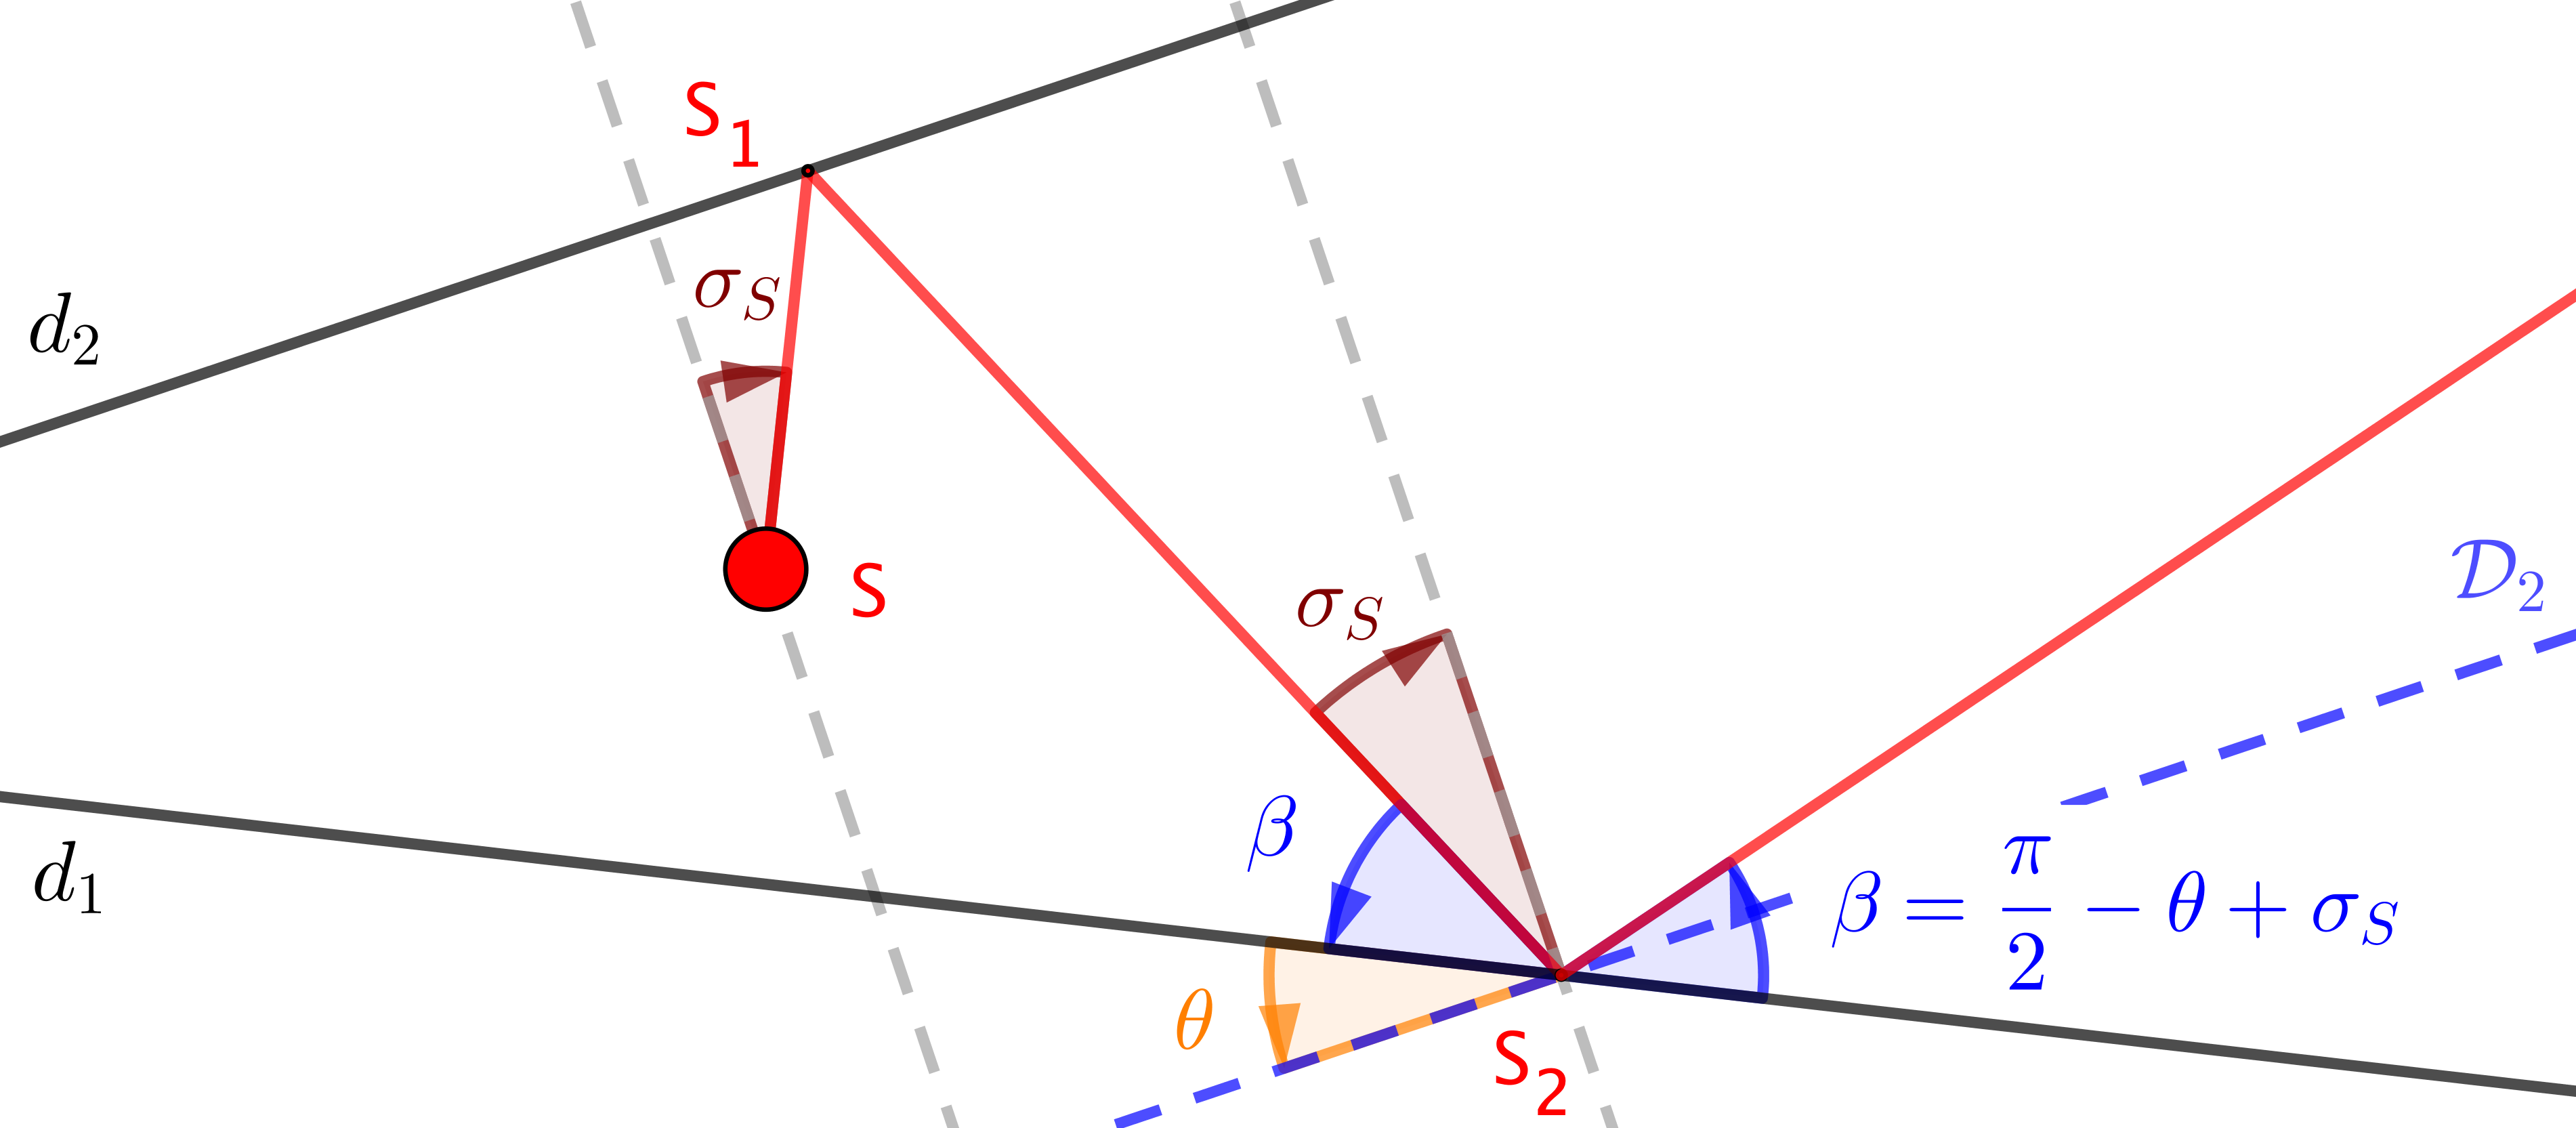
\includegraphics[width=12cm]{basic-math-pool/proof-starting-with-d2-2-bounces-farway-from-F-zoom.png}

	\itshape\small
	Preuve du fait \ref{s-eloigner} -- Vue zoomée du cas problématique
\end{center}
